\documentclass[conference]{IEEEtran}
\IEEEoverridecommandlockouts
% The preceding line is only needed to identify funding in the first footnote. If that is unneeded, please comment it out.
\usepackage{cite}
\usepackage{amsmath,amssymb,amsfonts}
\usepackage{algorithmic}
\usepackage{graphicx}
\graphicspath{images/}
\usepackage{textcomp}
\usepackage{xcolor}
\def\BibTeX{{\rm B\kern-.05em{\sc i\kern-.025em b}\kern-.08em
    T\kern-.1667em\lower.7ex\hbox{E}\kern-.125emX}}
\begin{document}

\title{Comparative Analysis of Deep Learning Models for Network Intrusion Detection Systems}

\author{\IEEEauthorblockN{Brenton Budler}
\IEEEauthorblockA{\textit{School of Computer Science and Applied Mathematics} \\
\textit{The Universiy of the Witwatersrand}\\
Johannesburg, South Africa \\
brentonbudler1@students.wits.ac.za}
\and
\IEEEauthorblockN{Ritesh Adjoodha}
\IEEEauthorblockA{\textit{School of Computer Science and Applied Mathematics} \\
\textit{The Universiy of the Witwatersrand}\\
Johannesburg, South Africa \\
ritesh.adjoodha@wits.ac.za}
}

\maketitle



\raggedbottom

\begin{abstract}
\noindet Detecting network intrusions is an imperative part of the modern cybersecurity landscape. Over the years, researchers have leveraged the ability of Machine Learning to identify and prevent network attacks. Recently there has been an increased interest in the applicability of Deep Learning in the network intrusion detection domain. However, Network Intrusion Detection Systems developed using Deep Learning approaches are being evaluated using the outdated KDD Cup '99 and NSL-KDD datasets which are not representative of real-world network traffic. Recent comparisons of these approaches on the more modern CSE-CIC-IDS2018 dataset, fail to address the the severe class imbalance which leads to significantly biased results. By addressing this class imbalance and performing an experimental evaluation of a Deep Neural Network, Convolutional Neural Network and Long Short-Term Memory Network on both a legacy dataset, the NSL-KDD, and a modern dataset, the CSE-CIC-IDS2018, this research provides deeper insights into the performance of these models in classifying network intrusions. The potential benefits of using a Sparse AutoEncoder to perform dimensionality reduction prior to model training are also explored. Preliminary results indicate that although the Deep Neural Network boasts the highest classification performance, the Convolutional Neural Network is the most efficient and the Long Short-Term Memory Network is the most reliable. Performing feature extraction using the Sparse AutoEncoder does not appear to improve model performance. 
\end{abstract}

\section{Introduction}
The use of the internet and other interconnected networks has grown exponentially in recent years. This rapid development of online technologies has, however, been accompanied by an equally rapid increase in cyberattacks. Globally, Cybersecurity Ventures predicts that cybercrimes will cost companies \$10.5 trillion by 2025. The \textit{Cost of Data Breach Report 2020} by researchers at IBM suggests that these devastating conequences are a result of cybersecuirty breachs taking an average of 280 days to identify and contain.

One solution to these constantly evolving attack scenarios is cybersecurity systems built on the foundations of Artificial Intelligence (AI) which can leverage the ability of Machine Learning (ML) to identify anomalies, detect and prevent these attacks. One such system is a Network Intrusion Detection System (NIDS) which monitors incoming and outgoing network traffic in an attempt to identify threats as depicted in Figure \ref{NIDS_implement}.
NIDSs are divided into two major categories; signature-based and anomaly-based \cite{b2}. Signature-based systems, also known as misuse-based systems, operate by comparing network traffic with a stored database of known attack patterns and flagging potential threats based on their similarity to these attacks \cite{b3}. The most prevalent drawback of signature-based systems is the inability to identify novel attacks \cite{b1}. The storing and maintaining of a database of all known attack patterns is also computationally expensive \cite{b4}.

On the other hand, anomaly-based systems first determine a benign network traffic baseline and then identify any network activity which deviates significantly from this baseline as a potential threat \cite{b5}. The ability of anomaly-based systems to identify unknown attacks has led it to become the most widely used approach in identifying network intrusions \cite{b6}.

\begin{figure}[htbp]
\centerline{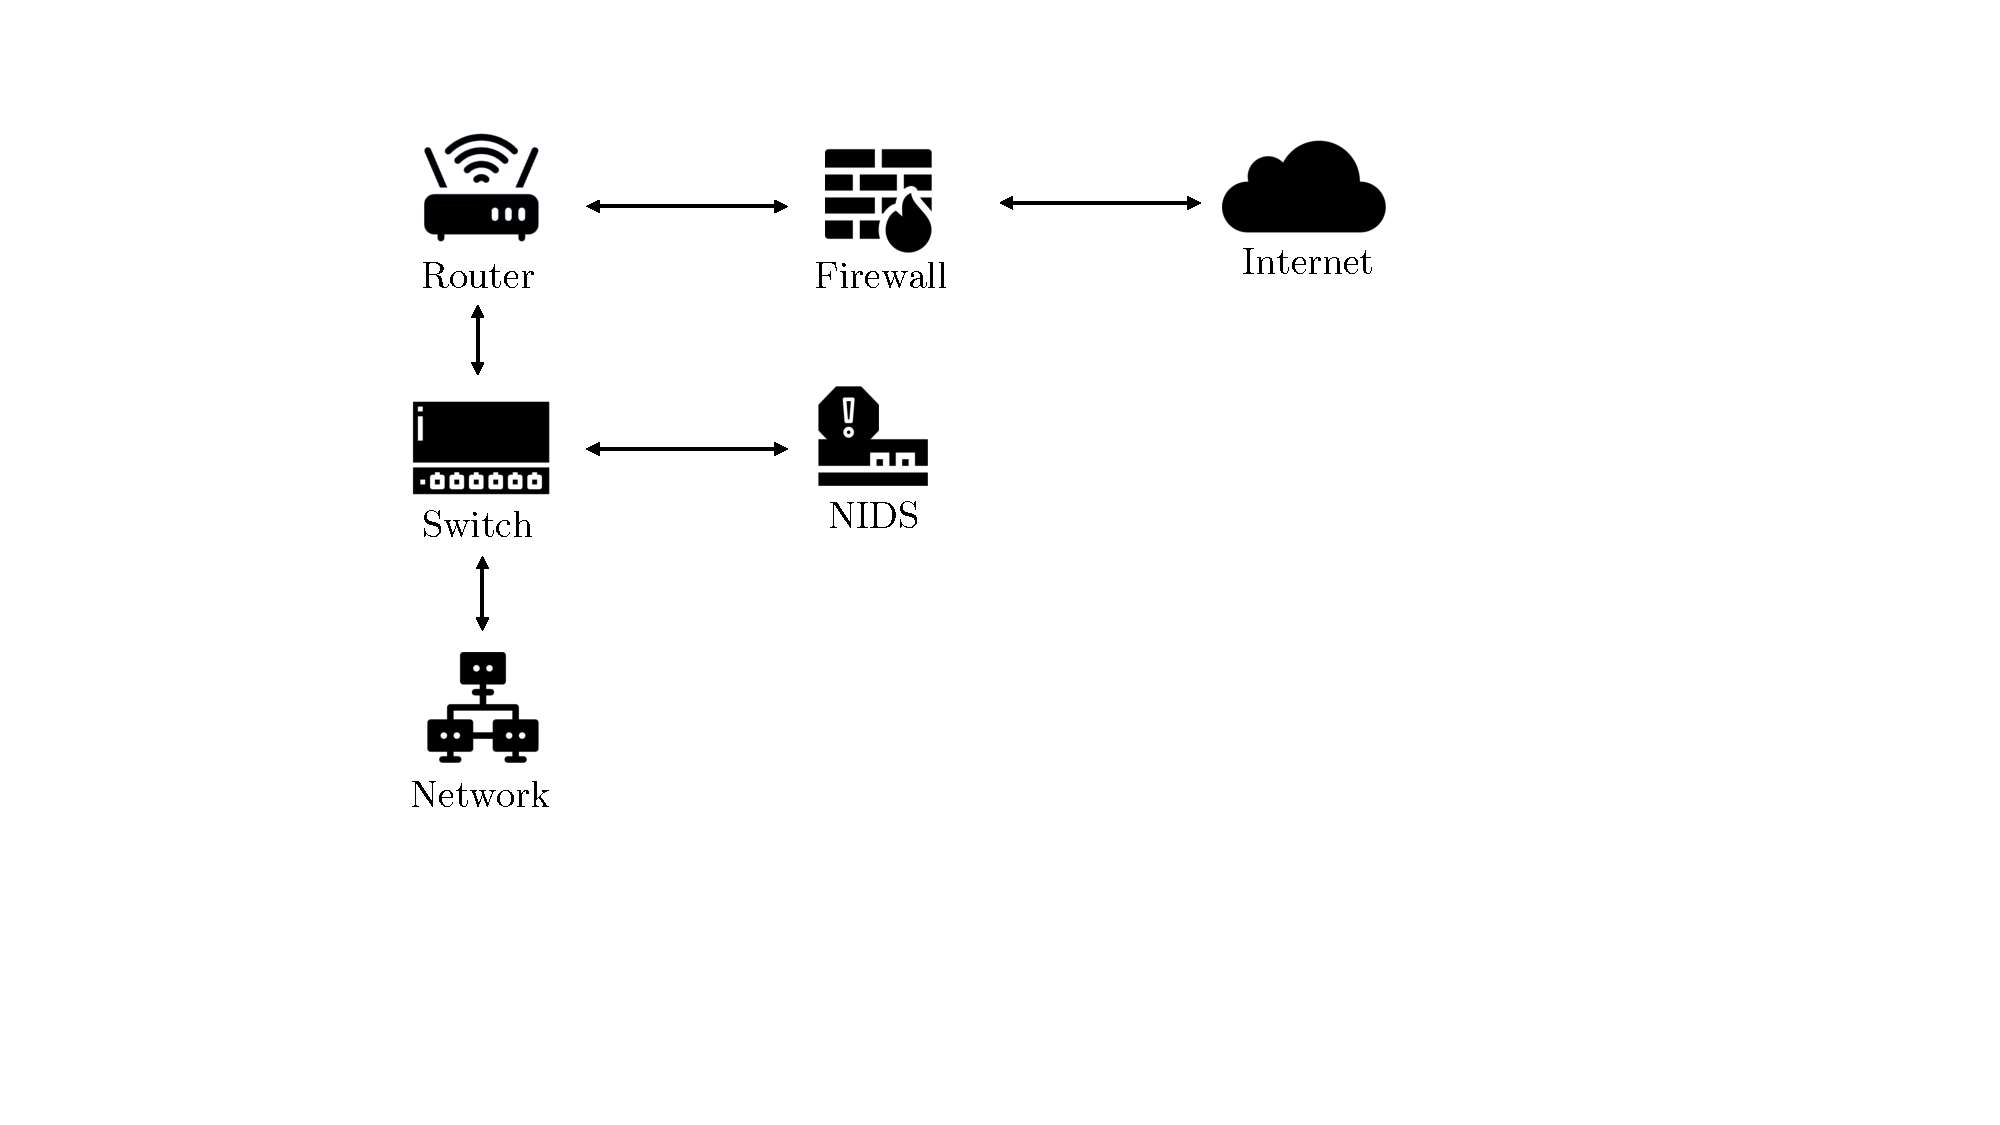
\includegraphics[scale=0.25]{images/diagram.pdf}}
\caption{Network Intrusion Detection System (NIDS) implementation}
\label{NIDS_implement}
\end{figure}

Recently, researchers have developed anomaly-based systems using ML techniques and have demonstrated the ability of these systems to efficiently solve the network intrusion detection problem\cite{b8}. The construction of these traditional ML models unfortunately relies heavily on feature engineering, a time-consuming task that requires domain expertise. \cite{b9}. 

Conversely, multi-layer Deep Learning (DL) models are capable of automatically extracting complex feature representations from data with little to no human interaction\cite{b10}. Research have demonstrated that
incorporating DL models, such as Deep Neural Networks (DNNs) and Convolutional Neural Networks (CNNs), into the development of NIDS results in faster and more accurate network intrusion detections, when compared to tradition ML approaches \cite{vin_make_poo, xiao}. The popular, two-stage Self-Taught Learning (STL) approach, has also shown promising results in the NIDS domain\cite{b2}. 

These approaches were, however, evaluated using outdated datasets which are not representative of modern network traffic, leading to disputable results. Recent comparisons of these approaches have been performed using more modern network traffic data, namely the CSE-CIC-IDS2018 dataset, but do not address the severe class imbalance in the data resulting in biased performance metrics. 

This research provides an experimental comparison of three popular DL approaches on both a legacy benchmark dataset, the NSL-KDD, and a modern dataset, the CSE-CIC-IDS2018. A Deep Neural Network (DNN), a Convolutional Neural Network (CNN) and a Long Short-Term Memory Recurrent Neural Network (LSTM) are evaluated using a number of performance metrics including accuracy, F1 Score, False Alarm Rate (FAR), model training time and inference time. An undersampling technique is used to address the class imbalance of the CSE-CIC-IDS2018 dataset, hereby ensuring unbiased results. To demonstrate the improvements offered by DL techniques in the NIDS domain, a traditional ML model, a Support Vector Machine (SVM),  is used as a benchmark in the comparison. 

The potential benefits of first using a Sparse AutoEncoder (SAE) to perform dimensionality reduction, as outlined in the STL approach, are also investigated for the DNN and CNN models. Furthermore, to investigate the generalizabity of these models across datasets, the same model architectures are used to evaluate these models on both the NSL-KDD and CSE-CIC-IDS2018 datasets. 

The contribution of this research is two-fold. Firstly, the experimental comparison provides deeper insights into the performance of DL models in detecting and classifying network intrusions. Secondly, by providing a clear outline of the data preprocessing techniques used and the implementation details of the models, this research presents unbiased and reproducible results which serve as a baseline for future research. These implementations are also made publicly available at $discord link$. 

Preliminary results indicate that there is a trade-off that exists between model classification performance and model efficiency as although the DNN was able to attain the highest Accuracy and F1 Score on both the NSL-KDD and CSE-CIC-IDS2018 datasets, the shared network parameters in the CNN architecture resulted in it having the shortest model training time and fastest inference time. The LSTM demonstrated the most consistent performance over multiple runs and the inclusion of the SAE for feature extraction did not demonstrate any significant improvements in the performance of the DNN or the CNN.

The rest of this report is structured as follows; Section II presents a brief review of approaches that have been used to develop and evaluate DL-based NIDS. Section III outlines the methodology used to conduct the experimental comparison including the datasets used, the preprocessing done to the data, the implementation details of the models, the metrics used to evaluate the models as well as the software and hardware that were utilized to develop the models. Section IV presents the results of the comparison and an interpretation of these results. Lastly, the report is concluded in Section V with a brief summary of the work and recommendations for future research. 

\section{Related Work}

\begin{table}[htbp]
\caption{Key contributions in the literature}
\begin{center}
\begin{tabular}{|p{1.5cm}|p{1.8cm}|p{1.5cm}|p{2.1cm}|}
\hline
\textbf{Author} & \textbf{Dataset} & \textbf{Model} & \textbf{Results}\\[2pt]
\hline

Javaid, 2016 \cite{b2}  & NSL-KDD & SAE + SMR&
Accuracy: 79.1\% Precision: 84.0\% Recall: 69.0\%  \\
& & &F1: 75.76\%
\\[5pt]
\hline
Alrawashdeh, 2016 \cite{b6} & KDD Cup ‘99 & DBN + LR & Accuracy: \textbf{97.9\%} Recall: 97.5\%\\[10pt]
\hline
Yin, 2017 & NSL-KDD & RNN&
Accuracy: 81.29\% \\[5pt]
\hline
Shone, 2018 \cite{b10} & NSL-KDD & NDAE + RF & 
Accuracy: \textbf{85.4\%} Precision: 100\% Recall: 85.42\% F1: 87.37\%\\
\hline 
Al-Qatf, 2018 & NSL-KDD & SAE + SVM & 
Accuracy: 80.48\% Precision: 93.92\% Recall: 68.25\% F1: 79.08\%\\
\hline
Vinayakumar, 2019 & NSL-KDD & DNN &
Accuracy: 78.5\%  Precision: 81.0\% Recall: 78.5\% \\
& & & F1: 76.5\% \\ 
\hline 
Xiao, 2019 & KDD Cup ‘99 & AE + CNN & 
Accuracy: 94\% Recall: 93\% \\
\hline 
\end{tabular}
\label{tab1}
\end{center}
\end{table}

As outlined in the introduction, the Self-Taught Learning (STL) framework has become a popular approach in NIDS research. This two-stage approach involves first learning an effective feature representation of the data using a large collection of unlabelled data, referred to as the Unsupervised Feature Learning (UFL) stage of the framework. In the second stage, the learnt feature representations are used as the input to a supervised algorithm which performs the classification task. The initial proposal of this framework, utilized a Sparse AutoEncoder (SAE) for UFL followed by a SoftMax Regression (SMR) for classification and was able to significantly improve the classification performance of a SMR on the NSL-KDD dataset\cite{b2} . 

Following the success of the STL framework, numerous researchers have experimented with different combinations of models to perform the feature extraction and classification tasks as outlined in Table I. The performance metrics in the table are for the five-class classification taks as the records in the KDD Cup '99 and NSL-KDD datasets are classified as either benign or as one of four attack types; User to Remote, Denial of Service , Probe or Remote to Local. The highest accuracy result for each dataset is emphasized. 

In\cite{b10}, the authors combined a Non-symmetric Deep AutoEncoder (NDAE) and Random Forest (RF) to perform the dimensionality reduction and classification respectively. They also included a model utilizing a Deep Belief Network (DBN) for feature extraction in their experimental evaluation, similar to the one incorporated in \cite{b6}, and demonstrated that their proposed model not only offered a 5\% improvement in accuracy on the NSL-KDD dataset but outperformed the DBN model across all performance metrics including precision, recall, F1-Score and False Alarm Rate (FAR). 

The STL approach was also implemented in \cite{al}, where a SAE is used for feature learning and a SVM is used to perform the classification task. The performance of the proposed model is compared with that of a vanilla SVM and beyond the improvements in classification accuracy, the STL approach also boasted a dramatic reduction in model training and inference times. These time reductions are imperative as timeliness is crucial when developing systems to detect network intrusions in real-world environments.

Model efficiency is improved even further by the work in \cite{xiao}. After reducing dimensionality using an AE, these authors transformed the data into a two-dimensional matrix and used this as the input to a CNN. The CNN performed further feature extraction and the classification task. The authors demonstrated the ability of their proposed model to classify the records of the NSL-KDD dataset more accurately and efficiently than a number of traditional and DL models including Logistic Regression (LR), RF, SVM, DNN and Recurrent Neural Network (RNN) on the KDD Cup '99 Dataset.

Instead of using separate models for feature extraction and classification, the authors in [yin] and [vin] use a DNN and a RNN respectively to extract better representations from the data and perform the classification task. Both these papers demonstrate the ability of these DL models to outperform traditional ML approaches on the NSL-KDD dataset but neither include other DL techniques in their evaluations, highlighting the lack of an objective comparison of DL approaches in the literature. 

% The aforementioned models use DL for 

% Although a number of the aformentioned models use DL for pre-training only, performing classification using traditional supervised models, a Recurrent Neural Network (RNN) is used to extract better representation from the data and perform the classification in \cite{b8}. The classification ability of the RNN demonstrated an increased accuracy and lower False Alarm Rate (FAR) on the NSL-KDD dataset when compared to several traditional supervised algorithms. 

% Vinayakumar also used one network, a Deep Neural Network (DNN), to perform both the feature extraction and classification tasks on a number of IDS datasets. In all cases the DNNs exceeded the performance of classical machine learning classifiers. Evidently both these papers compare their results with traditional machine learning approaches resulting in a lack of an objective comparison of different DL approaches. \\ 

The primary disadvantage of the papers outlined above is the utilization of the KDD Cup '99 and NSL-KDD datasets when evaluating model performance. Network architectures have changed dramatically over the past 20 years and these older datasets no longer represent modern attack styles \cite{b4}. Researchers continue to validate their use of these older datasets with the fact that it allows them to draw comparisons with other academic literature \cite{b10} but if future researchers continue using only these datasets to evaluate their work, their conclusions will only become more disputable. 

% NIDS methodologies proposed using these datasets have also been shown to perform poorly when deployed in the modern real-world cybersecurity environment \cite{b12}.

In order to address the lack of an empirical comparison of DL models for network intrusion detection on newer datasets, researchers have recently begun performing comparisons of these models on the CSE-CIC-IDS2018 dataset. Their results are summarized in Table 2 and a brief review of their work is included below.

\begin{table}[htbp]
\caption{Deep Learning Model Comparisons}
\begin{center}
\begin{tabular}{|p{1.7cm}|p{2cm}|p{3.5cm}|}
\hline
\textbf{Author} & \textbf{Model} & \textbf{CSE-CIC-IDS2018 Results}\\[2pt]
\hline
Ferrag, 2020 & DNN & Accuracy: 97.281\%\\[2pt]
 & RNN & Accuracy: 97.310\%\\[2pt]
 & CNN & Accuracy: \textbf{97.376\%}\\[2pt]
 & RBM & Accuracy: 97.280\%\\[2pt]
 & DBN & Accuracy: 97.302\%\\[2pt]
 & DBM & Accuracy: 97.371\%\\[2pt]
 & DAE & Accuracy: 97.372\%\\[2pt]
\hline 
Gamage, 2020 & DNN & Accuracy: \textbf{98.38}\%\\[2pt]
 & AE + DNN & Accuracy: 98.22\%\\[2pt]
 & DBN + DNN & Accuracy: 98.31\%\\[2pt]
 & LSTM & Accuracy: 97.60\%\\[2pt]
\hline
\end{tabular}
\label{tab1}
\end{center}
\end{table}

In \cite{b13}, the authors utilize the taxonomy presented by Deng and Yu \cite{b23} to classify deep learning approaches into two categories; deep discriminative models and generative/unsupervised models. The models they select for their comparison include a RNN, a DNN and a CNN (deep discriminative models) as well as a Deep AE, a Restricted Boltzmann Machine , a Deep Boltzmann Machine and a DBN (generative/unsupervised models). Although their comparison includes a wide variety of models, it contains very little information about data pre-processing and does not provide details about the model architectures and hyperparameters used.

A new taxonomy of DL models for network intrusion detection is proposed by the authors in \cite{b14}. Their taxonomy divides models into 4 categories namely; supervised instance learning, supervised sequence learning, semi-supervised instance learning and other learning paradigms. In their evaluation, a DNN is selected to represent the first category, an LSTM to represent the second and an AE as well as a DBN to represent the third. The authors believe these models are representative of the different approaches for building DL models, but their evaluation is undermined by the fact that they do not include a CNN in their comparison, which the authors in \cite{b13} found to be the best performing model on the CSE-CIC-IDS2018 dataset. However, a significant result found in this comparison is that the inclusion of an AutoEncoder
to perform dimensionality reduction was unable to improve the classification performance of the DNN. 

The major downfall of both these comparisons is that they do not address the high class imbalance present in the CSE-CIC-IDS2018 dataset. This high class imbalance makes the identification of minority classes by DL models difficult and introduces bias in favour of the majority classes resulting in deceptively high performance metrics \cite{b17}. 

In order to ensure the results from the comparison in this research were not biased by the class imbalance, an undersampling technique, which ensures an equal class distribution, was incorporated in the preprocessing of the CSE-CIC-IDS2018 dataset. Furthermore, to ensure the comparison is representative of the best performing models found in prior works, the empirical comparison includes a DNN, a CNN , and a LSTM.  


\section{Methodology}

The Related Work section above identified a number of shortfalls found in the literature. The list below outlines how each of these shortfalls were addressed in this research. 

\begin{itemize}
    \item \textbf{The use of outdated datasets:} The NSL-KDD dataset was used purely to verify that the models were implemented correctly and attained results similar to those reported in the literature. Thereafter the models were evaluated using the modern CSE-CIC-IDS2018 dataset. 
    \item \textbf{Not addressing the class imbalance of the CSE-CIC-IDS2018 dataset:} An undersampling technique which ensures an equal class distribution was incorporated into the preprocssing of the CSE-CIC-IDS2018 dataset. 
    \item \textbf{Unrepresentative model selection:} In order to ensure that the comparison is representative of all categories across both taxonomies presented in the literature a DNN, a CNN, a LSTM as well as a DNN and CNN which use a SAE for dimensionality reduction are included in the comparison. The SAE is used inplace of the DBN as prior work demonstrated the superior performance of the AE and its variants to perofrm feature extraction. \cite{b10,b13,b14}
    \item \textbf{Not providing information about data preprocessing, model architectures and hyperparameters:} The data preprocessing procedure used for both the NSL-KDD and CSE-CIC-IDS2018 dataset, the model architectures and hyperparemters are all delineated below. 
\end{itemize}

% % rewrite this to incorporate what we have learnt from related work section 
% % The models are first evaluated using the NSL-KDD dataset, this is done purely to verify that the models have been implemented correctly and attain similar results to those reported in the literature. Thereafter the models are evaluated using the undersampled CSE-CIC-2018IDS dataset. ]

% To explore the potential improvements offered by the popular two-stage approach found in the literature, three models which use a SAE to perform dimensionality reduction are also included in a separate comparison. One of these models performs the classification using a SVM, one uses a DNN and the other uses a CNN. The SAE is used in favour of the DBN as prior work demonstrates the superior performance of the AE and its variants, for feature extraction \cite{b10,b13,b14}. Including these  models ensures that all categories across both taxonomies are represented in the comparison.  \\


\subsection{Data}\label{AA}

\subsubsection{NSL-KDD Dataset}
As noted in the Related Work section , the two most used datasets in NIDS research are the KDD Cup ’99 and the NSL-KDD datasets. The KDD Cup ’99 dataset was generated in 1999 from the DARPA98 network traffic which was collected over 9 weeks in raw tdpdump format \cite{b2}. The KDD Cup ’99 has been used as a benchmark in NIDS research for many years but suffers from the major drawback that about 75\% of the records are redundant. The NSL-KDD dataset was derived from the original KDD Cup ’99 dataset and effectively solved the inherent redundant record problem \cite{b8}. It also partitioned the records into different difficulty categories based on the number of traditional ML algorithms that were able to correctly classify the records.
The NSL-KDD dataset consists of 41 network traffic features which contain both host-based and time-based information.\\

\subsubsection{CSE-CIC-IDS2018 Dataset}
\noindent The CSE-CIC-IDS2018 is a collaborative project between the Communications Security Establishment (CSE) and the Canadian Institute of Cybersecurity(CIC). The CSE-CIC-IDS2018 is the most recent network intrusion detection dataset that is publicly available, contains a wide range of attack types and consists of enough network traffic to be considered big data \cite{b17}. It was developed as a comprehensive and diverse benchmark dataset for network intrusion detection, specifically anomaly-based methods \cite{b16}. The dataset contains 16,233,002 instances of network traffic captured over the course of 10 days. Seven different attack scenarios are represented in the dataset; Denial-of-Service (DoS), Distributed Denial-of-Service (DDoS), Brute-force, Heartbleed, Botnet and inside infiltration. The dataset consists of 80 features extracted from the raw network data by the CICFlowMeter-V3, a network traffic flow analyser \cite{b16}.

% As previously noted, a prevalent issue in the CSE-CIC-IDS2018 is the severe class imbalance. Whilst many researchers do not address this class imbalance , \cite{b18} overcome it using the Focal Loss Function while \cite{b19} address it using Synthetic Minority Oversampling Technique (SMOTE). 

\subsection{Data Preprocessing}
\subsubsection{NSL-KDD}
\noindeny The NSL-KDD dataset is provided as two separate csv files, one containing the data for model training and one containing testing data. The files contain a total of 43 columns, including the 41 features, an attack type label and a difficulty level. Due to the way the difficulty level was derived it was removed from the dataset. The ‘num\_outbound\_calls’ feature was also removed as it only contains the value zero for all records and would not contribute to the classification ability of the models. The dataset originally contains 23 different categories for the attack type label which are grouped into 5 different attack classes for the classification task as outlined in Table III below.
The features indicating the protocol type used in the connection, the destination service used and the status of the connection are all categorical features with 3, 70 and 11 categories respectively. These categorical features are one-hot encoded, yielding a total of 121 features, and 1 attack type class label.
Although the dataset is already divided into training and testing data by the providers, 20\% of the training data is used as validation data for hyperparameter tuning. 


\begin{table}[htbp]
\caption{NSL-KDD Class Distribution}
\begin{center}
\begin{tabular}{|p{1.75cm}|p{1cm}|p{1cm}|p{1cm}|p{1cm}|}
\hline
\textbf{Class} &
\multicolumn{2}{|c|}{\textbf{Records}} &
\multicolumn{2}{|c|}{\textbf{Percentage of data}}
\\
\cline{2-5}
 & \textit{Train}& \textit{Test}&\textit{Train}& \textit{Test}\\[2pt]
\hline
Benign & 67 343 & 9711 & 53.458\% & 43.076\% \\[5pt]
\hline
Dos Attack & 45 927 & 7460 & 36.458\% & 33.091\% \\[5pt]
\hline
Probe Attack & 11 656 & 2421 & 9.253\% & 10.739\% \\[5pt]
\hline
U2R Attack & 52 & 67 & 0.041\% & 0.297\% \\[5pt]
\hline
R2L Attack & 995 & 2885 & 0.790\% & 12.797\% \\[5pt]
\hline
\end{tabular}
\label{tab1}
\end{center}
\end{table}


\subsubsection{CSE-CIC-IDS2018}
\noindent The CSE-CIC-IDS2018 dataset is provided as 10 files corresponding to the 10 day period over which the network traffic was captured. In order to reduce computational costs, instead of processing the entire dataset at once, these 10 files were partitioned according to the attack type which was being simulated on that day as outlined in Table IV below. Each partition of the dataset was preprocessed in the same way with records containing missing or erroneous values being removed and the protocol type feature being one-hot encoded. \\

\begin{table}[htbp]
\caption{CSE-CIC-IDS2018 Partition Class Distribution}
\begin{center}
\begin{tabular}{|p{1.25cm}|p{2cm}|p{2cm}|p{2cm}|}
\hline
\textbf{Partition} & \textbf{Files Included} &
\multicolumn{2}{|c|}{\textbf{Attack Records}} \\[15pt] %\textbf{Percentage of dataset}% 
\cline{3-4}
 & & \textit{Before Cleaning}& \textit{After Cleaning}\\[15pt]
\hline
BruteForce & 02-14-2018.csv & 380 949 & 156 668 \\[5pt] %& 2.347\%
\hline 
DoS & 02-15-2018.csv, 02-16-2018.csv &
654 300 & 506 075 \\[5pt] %& 4.031\%
\hline
Web & 02-22-2018.csv, 02-23-2018.csv &
928 & 928 \\[5pt] %& 0.006\%
\hline
Infiltration & 02-28-2018.csv, 03-01-2018.csv &
161 934 & 135 270 \\[5pt] %& 0.997\%
\hline 
Botnet  & 03-02-2018.csv &
1 263 933 & 1 246 366 \\[5pt] %& 1.763\%
\hline
DDoS & 02-20-2018.csv, 02-21-2018.csv &
1 263 933 & 1 246 366 \\[5pt] %& 7.786\%
\hline
\end{tabular}
\label{tab1}
\end{center}
\end{table}

As previously noted, an undersampling technique was utilized to address the heavy class imbalance present in the CSE-CIC-IDS2018 dataset. This undersampling technique involved identifying the attack class with the least number of records in the dataset and then randomly selecting the same number of records for each of the other attack classes. The least frequent attack type class in the dataset after removing duplicates and missing data was the Web Attack class with 928 records, this meant that 928 attack records were selected from each partition. Benign records were then selected from each partition according to the proportion of total benign records in the original dataset that partition contained. 

Unlike the NSL-KDD which is already split into training and testing data, the CSE-CIC-IDS2018 dataset needs to be divided. 60\% of the undersampled data is used for training, 20\% is used for validation and 20\% is used for evaluation. This split was done in a stratified manner, to ensure the distribution of the target class was similar in each subset of data. 

The incorporation of the CNN model requires further preprocessing as the one-dimensional network traffic data needs to be transformed into the two-dimensional matrix form, required for the input of the CNN. For the NSL-KDD dataset, each record is represented by a feature vector with 121 features and could therefore be transformed into an 11x11 image. After preprocessing the CSE-CIC-IDS2018 contained 79 features, due to its prime nature this number of features could not inherently be transformed in the same way. Therefore two features, containing all zeros, were added to the CSE-CIC-IDS2018 dataset, this allowed the records to be transformed into 9x9 images without effecting the classification ability of the DL models used in the comparison. Figure \ref{nsl_class} and Figure \ref{cic_class} contain examples of the newly formed two-dimensional input images for both datasets. 

% \noindent Both the NSL-KDD and CSE-CIC-IDS2018 were both scaled using minimum-maximum normalization prior to model training and evaluation. 


\begin{figure*}[htbp]
\centerline{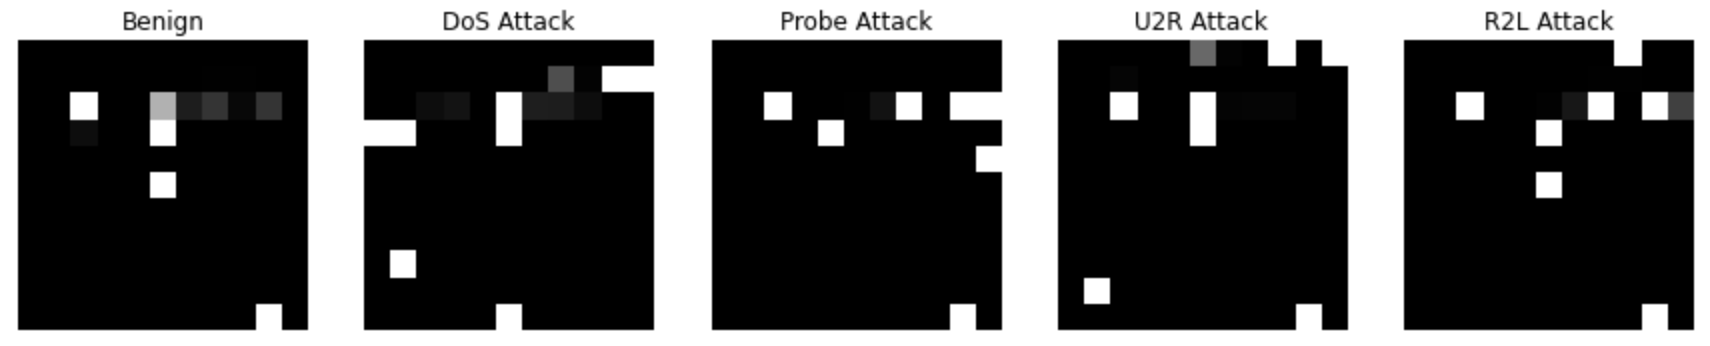
\includegraphics[scale=0.5]{images/nsl_kdd_classes.png}}
\caption{NSL-KDD Example Two-dimensional Image Data}
\label{nsl_class}
\end{figure*}

\begin{figure*}[htbp]
\centerline{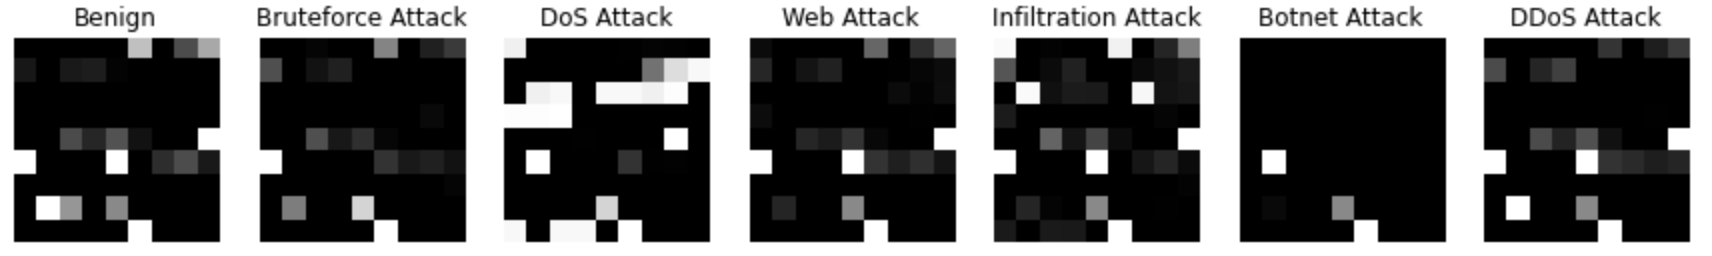
\includegraphics[scale=0.5]{images/cic_cse_classes.png}}
\caption{CSE-CIC-IDS2018 Example Two-dimensional Image Data}
\label{cic_class}
\end{figure*}



\subsection{Models}

\begin{table}[htbp]
\caption{Hidden Layer Architecture for Models}
\begin{center}
\begin{tabular}{|c|c|}
\hline
\textbf{Model} & \textbf{Hidden Layer Architecture}\\[2pt]
\hline
DNN & Fully Connected -  64 Neurons\\[2pt]
    & Batch Normalization\\[2pt]
    & Dropout - $p=0.2$\\[2pt]
    & Fully Connected -  32 Neurons\\[2pt]
    & Batch Normalization \\[2pt]
    & Dropout - $p=0.2$ \\[2pt]
    & Fully Connected -  16 Neurons\\[2pt]
    & Batch Normalization \\[2pt]
    & Dropout - $p=0.2$ \\[2pt]
    
\hline 
CNN & Convolution -  8 filters , 2$\times$2 kernel\\[2pt]
    & Batch Normalization\\[2pt]
    & MaxPool - 2$\times$2 pool size\\[2pt]
    & Convolution -  16 filters , 2$\times$2 kernel\\[2pt]
    & MaxPool - 2$\times$2 pool size\\[2pt]
    & Dropout - $p=0.2$ \\[2pt]
    & Fully Connected -  64 Neurons \\[2pt]
\hline 
LSTM & Fully Connected LSTM-  64 Neurons\\[2pt]
    & Batch Normalization\\[2pt]
    & Dropout - $p=0.2$\\[2pt]
    & Fully Connected LSTM-  32 Neurons\\[2pt]
    & Batch Normalization \\[2pt]
    & Dropout - $p=0.2$ \\[2pt]
\hline
\end{tabular}
\label{tab1}
\end{center}
\end{table}

The initial implementation of each model was done using the model architectures and hyperparameter values reported by the authors who originally proposed the models in prior work. Further hyperparameter tuning was performed experimentally by observing the effect of varying model architectures and hyperparameters on the performance metrics of each model. Table V contains a detailed breakdown of the hidden layer architectures used for each model, the number of input neurons was determined by the input features of each dataset whilst the number of neurons in the output layer coincides with the number of target classes in the dataset.

To reduce the possibility of overfitting when training the models, early stopping, a form of regularization which stops training once the model performance on an unseen subset of data (the validation set) stops improving, was included in the training process.  The validation loss was monitored and if no improvement is detected for 5 epochs, training was stopped and the best performing network weights were restored. With the incorporation of early stopping, the number of epochs that each model should train for did not need to be explicitly set as a hyperparameter, as it varied depending on the number of epochs required for the validation loss to reach convergence. To ensure any variance in the training processes, including the variance caused by randomly splitting data, was accounted for, the training and evaluation process for each model was repeated five times, with all reported metrics being the mean of the five iterations. 

In order to accelerate training, a batch size of 256 records was utilized along with Batch Normalization. Batch Normalization is an optimization method proposed by Google in which each batch of data used in training is standardized before being fed to the next layer in the network, hereby stabilizing and accelerating training. 

Dropout, another regularization technique presented by Hinton \cite{b23}, was also used to further reduce the risk of overfitting in the model training process. This technique involves randomly setting the weights of some hidden layer neurons to zero, temporarily excluding those neurons from the training calculations hereby preventing the development of unwanted co-dependencies between neurons. The dropout parameter $p$ indicates the probability that a neuron will be excluded at each step of training and was set to 0.2, as prior research indicates this is the optimal value for reducing overfitting without hindering model performance \cite{b14}.

The SAE, a variant of the AE, that introduces a sparse penalty to ensure the AE learns a more concise and efficient low-dimensional feature representation was used for feature reduction in the STL models. The sparsity parameter was set to 0.2 as the authors in [alwatf] experimentally evaluated the effect that varying the sparsity parameter had on model performance and demonstrated that a value of 0.2 could increase model accuracy and reduce model training time.  

% Figure [label] indicates the experimental procedure implemented to choose the number of features the sparse AutoEncoder would reduce the dataset to. By using different numbers of features and observing the effect this had on the baseline models perfromance. 
%Speak about the way you used autoencdoer for dimensionality reduction here as well as the sparse auto encoder thing and the training of an AE and all of that also give deatils about AE like 25% for training and reduced the dimension from 121 to 64 and 80 to 64 , variance reduction amount, maybe plot the accuracy using the different reduced dimensionality and say why you seleceted it, oh use the SVM to select the dimensions.%

\subsection{Evaluation Metrics}
The metrics used when evaluating the performance of a DL-based Network Intrusion Detection System are based on the different attributes found in a Confusion Matrix, a two-dimensional matrix which contains information about the actual classes and predicted classes for each instance in the dataset. Each instance is categorized into one of the following four categories:\\

\noindent i. \emph{True Positive (TP)} - An attack instance has been correctly classified as an attack\\ 
ii. \emph{False Positive (FP)} - A benign instance has been incorrectly classified as an attack\\
iii. \emph{True Negative (TN)} - A benign instance has been correctly classified as benign \\
iv. \emph{False Negative (FN)} - An attack instance has been incorrectly classified as benign \\

\noindent A number of useful performance measures can be derived from the Confusion Matrix to better gauge the performance of a DL-based NIDS.

\begin{table}[htbp]
\caption{Confusion Matrix}
    \centering
    
\begin{tabular}{cc|cc}
\multicolumn{2}{c}{}
            &   \multicolumn{2}{c}{\textbf{Predicted}} \\
            
    &       &   Attack &   Benign              \\ 
    \cline{2-4}
\multirow{\rotatebox[origin=c]{90}{\textbf{Actual}}}
    & Attack   & \emph{True Positive}   & \emph{False Negative}                 \\
    & Benign    & \emph{False Positive}    & \emph{True Negative}                \\ 
    \cline{2-4}
\end{tabular}

    
    \label{tab:my_label}
\end{table}
\\

\begin{itemize}
    \item \textbf{Accuracy:} Defined as the number of correctly classified instances over the total number of instances, accuracy represents the systems ability to correctly identify benign and attack instances. 
    
    \begin{equation}\label{eq1}
        Accuracy= \frac{TP + TN}{TP + TN + FP + FN}
    \end{equation}
    
    \item \textbf{Recall:} Also known as the Detection Rate (DR) or the True Positive Rate (TPR), recall is the number of correctly identified attacks over the total number of attack instances.
    
    \begin{equation}\label{eq2}
        Recall = Detection\:Rate = \frac{TP}{TP + FN}
    \end{equation}
    
    \item \textbf{Precision:} Represents how many of the instances identified as attacks were actually attacks, it is defined as the number of correctly identified attacks over all instances classified as attacks.
    
    \begin{equation}\label{eq3}
        Precision =  \frac{TP}{TP + FP}
    \end{equation}
    
    \item \textbf{F1-Score:} The harmonic mean between the recall and the precision which serves as a derived effectiveness measurement. 
    
    \begin{equation}\label{eq3}
        F-Score =  \frac{Recall \times Precision}{Recall + Precision}
    \end{equation}
    
    \item \textbf{False Alarm Rate:} Measures the portion of benign instances which were incorrectly classified as attacks.
    
    \begin{equation}\label{eq3}
        False\:Alarm\:Rate =  \frac{FP}{FP+TN}
    \end{equation}
    
\end{itemize}


\begin{figure*}[htpb]
  \centering
  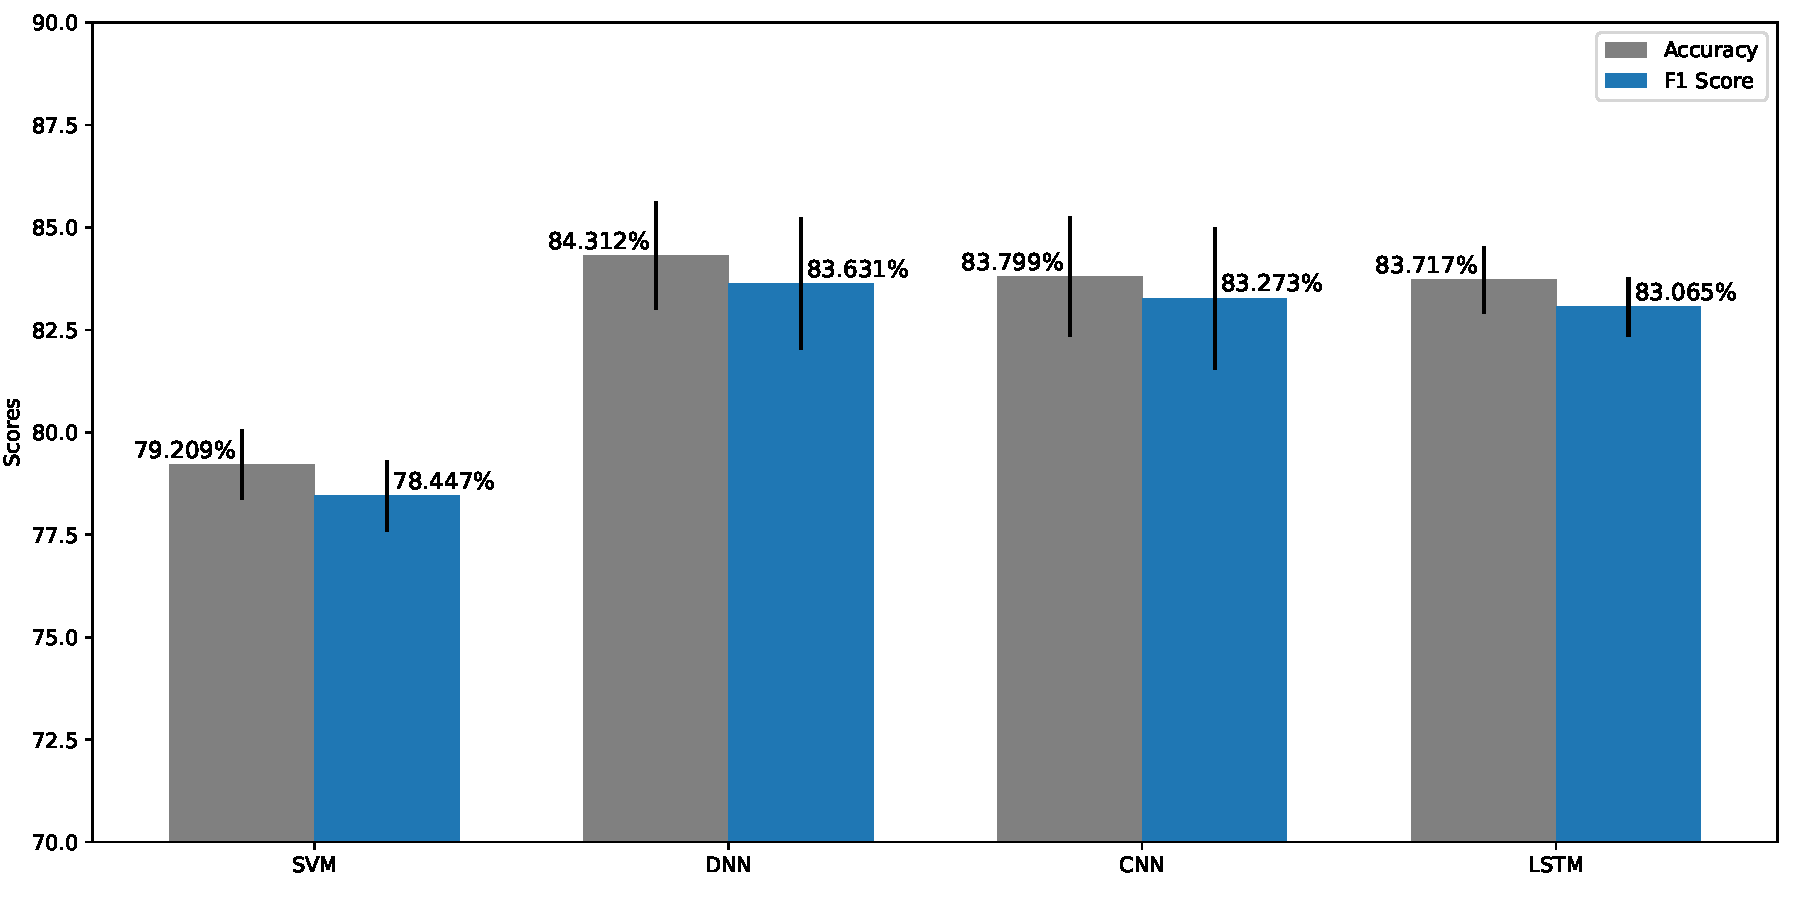
\includegraphics[width=0.75\textwidth]{images/acc_f1_cic.pdf}
  \caption{Model Classification Performance on Undersampled CSE-CIC-IDS2018}
  \label{fig:acc_f1_cic}
\end{figure*}

The objective of a NIDS is to obtain a high accuracy and F1-Score with a low False Alarm Rate \cite{b8}. These three indicators are used most often to evaluate NIDS systems \cite{b12} and are therefore the primary evaluation metrics used to empirically evaluate and compare models in this research. The problem in NIDS development is, however, two-fold. Not only do the performance metrics need to demonstrate that the model is effective but the model also has to be efficient because as previously noted, timeliness is critical in modern NIDS development. Thus, along with the performance metrics outlined above, the comparative analysis includes an examination of the time required to train each of the models as well as the time it took each model to make inferences about the testing data. 

\subsection{Software and Hardware}
In order to ensure a fair comparison of the different DL models, each model was constructed, trained, tested and evaluated on the same computing device using the same software frameworks. Model construction was done using Python with the TensorFlow and Keras frameworks \cite{b17}. A 13-inch Apple M1 MacBook Pro with 8GB RAM was used to carry out the experimental evaluation. 

% \begin{table}[htbp]
%     \centering
%     \caption{Device Specifications}
%     \begin{tabular}{|1|1|}
%         \hline
%              \multicolumn{2}{|c|}{\textbf{13-inch Apple M1 MacBook Pro}}\\
%         \hline
%              \textbf{Processor} &  M1 8-core  \\
%         \hline
%             \textbf{Storage} &  512GB \\
%         \hline
%             \textbf{RAM} &  8GB \\
%         \hline
%             \textbf{Graphics} &  Integrated 8-core GPU \\
%         \hline
%             \textbf{Neural Engine} &  Integrated 16-core \\
%          \hline
%     \end{tabular}
    
%     \label{tab:my_label}
% \end{table}

\section{Results}


\subsection{Verification of Model Implemnetation}

To verify the implementation of the models used in this comparison, the results attained on the benchmark dataset, the NSL-KDD, in prior works were compared to the results achieved in this evaluation. As evident in Table VIII, the classification performance of these models was very similar (within 3\%) of the results found in the literature. These minor disparities can be attributed to difference in preprocessing techniques and the variance associated with training neural networks. 

\begin{table}[htbp]
    \centering
    \caption{NSL-KDD Result Comparison with prior work}
    \begin{tabular}{|1|1|1|}
    
        \hline
             \textbf{Model} &  \textbf{Prior Work} & \textbf{This Work}  \\[10pt]
        \hline
            DNN &  77.26\% \cite{b14} &  76.127\% \\[5pt]
        \hline
            CNN &  NA & 74.101\% \\[5pt]
        \hline
            LSTM &  77.26\% \cite{b14} & 76.132\%\\[5pt]
        \hline
    \end{tabular}
    
    \label{tab:my_label}
\end{table}


%Insert table of conmparison here%

\subsection{Comparing Model Classification Performance}
As previously noted, in order to account for any variance in the datasplitting and model training processes, each model is trained and evaluated five times, with the reported metrics being the mean of the five iterations and the error bars on the plots below representing a single standard deviation, calculated over the five runs. 

As evident in Figure \ref{fig:acc_f1_cic}, all three Deep Learning models were able to outperform the classification performance of the traditional Machine Learning model, the SVM. Although the DNN was able to attain the highest average accuracy and F1-score , the LSTM achieved the lowest variance across multiple runs. By reducing the number of neruons from hidden layer to hidden layer in the DNN, the model is able to learn complex features and extract better representations of the data which in turn can be used to make more accurate classifications. The low variance of the LSTM  model is a result of the feedback loop incorporated in the architecture of LSTMs which is capable of memorizing previous information and applying it to the current output. This allows it to learn long term dependencies in the network data and reduce the variability of the run-to-run classification performance. The transformation of the network traffic data into two-dimensional images and the utilization of a CNN to classify these image data does not appear to improve classification performance. Due to the fact that the network traffic data does not inherently contain any spatial information, the positional relation of the features in the two-dimensional form does not appear to provide the model with any useful additional information resulting in similar performance to the other neural networks.



\begin{figure}[!htpb]
  \centering
  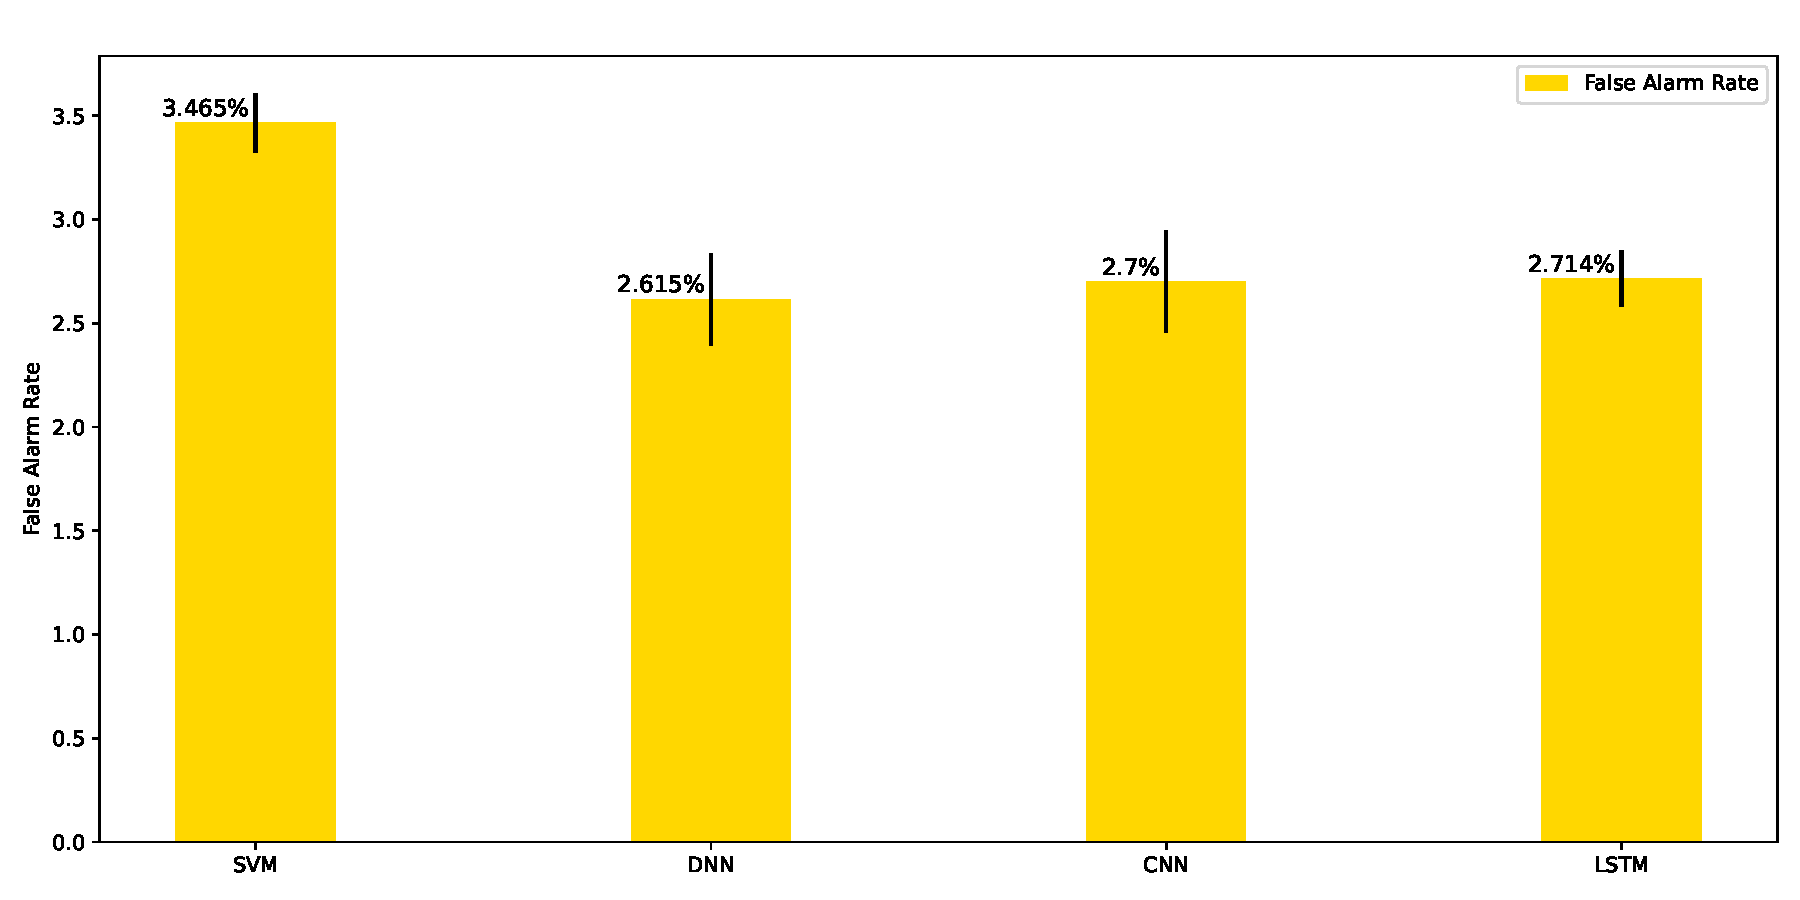
\includegraphics[width=0.4\textwidth]{images/far_cic.pdf}
  \caption{Model False Alarm Rate on Undersampled CSE-CIC-IDS2018}
  \label{fig:far_cic}
\end{figure}

Once again in figure \ref{fig:far_cic}, it can be observed that all three of the deep learning models were able to reduce the False Alarm Rate on the Undersampled CSE-CIC-IDS2018 dataset, when compared to the shallow learning baseline. The lowest FAR is attained by the DNN whilst the lowest variance in run-to-run performance is achieved by the LSTM, which coincides with the observations made above and reaffirms the corresponding interpretation. 

\subsection{Comparing Model Efficiency}

\begin{figure}[htpb]
  \centering
  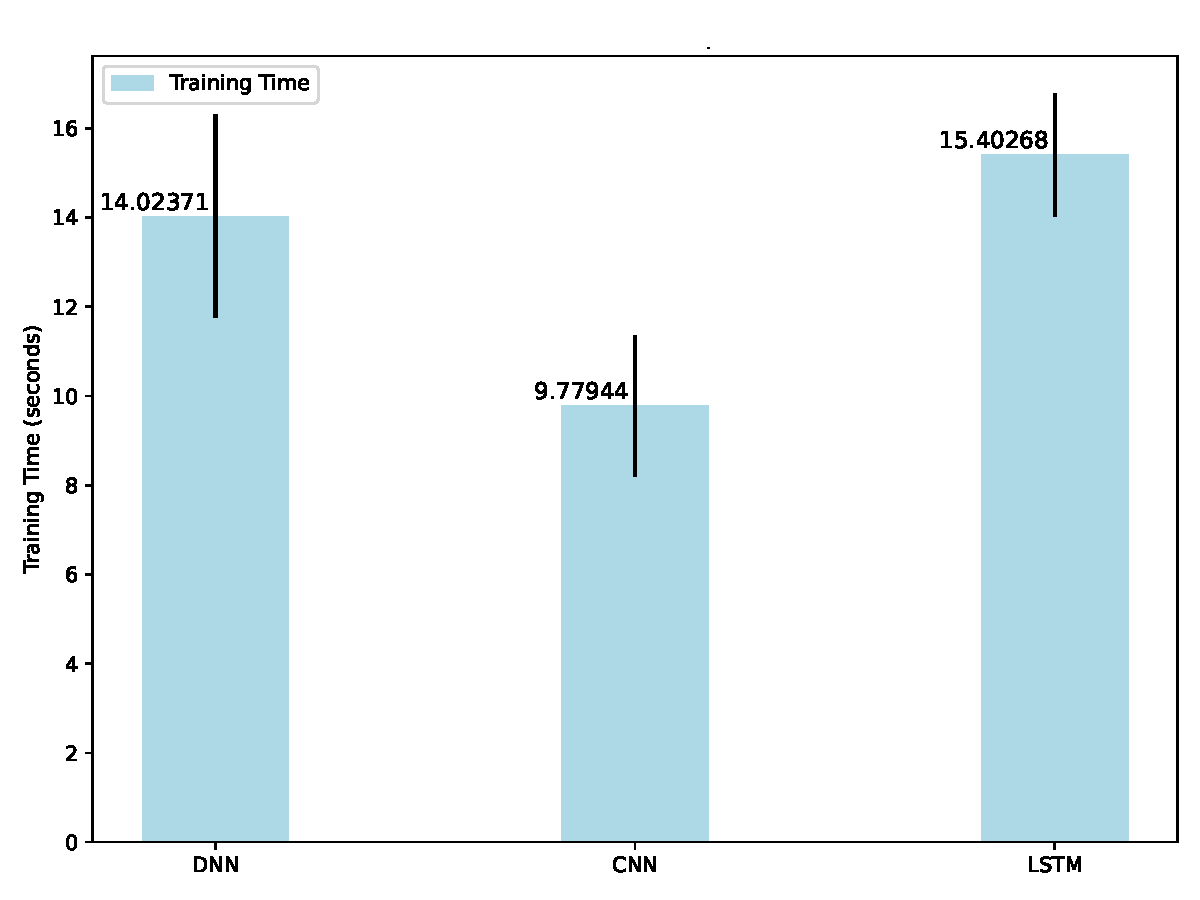
\includegraphics[width=0.35\textwidth]{images/train_time_cic.pdf}
  \caption{Model Training Time on Undersampled CSE-CIC-IDS2018}
  \label{fig:train_time_cic}
\end{figure}

\begin{figure}[htpb]
  \centering
  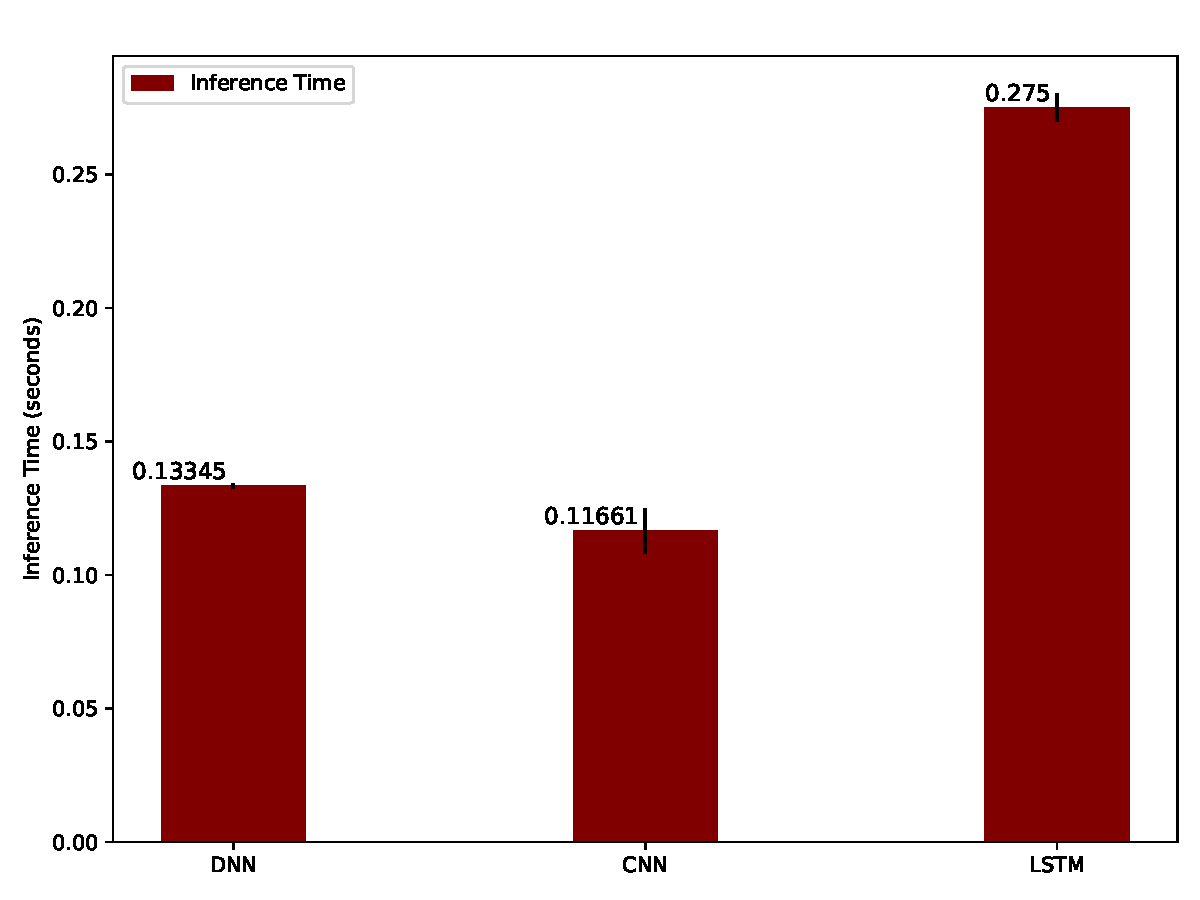
\includegraphics[width=0.35\textwidth]{images/test_time_cic.pdf}
  \caption{Model Inference Time on Undersampled CSE-CIC-IDS2018}
  \label{fig:test_time_cic}
\end{figure}


The results in Figure \ref{fig:train_time_cic} and Figure \ref{fig:test_time_cic} reveal that there is a trade-off that exists between model accuracy and model efficiency. Although the CNN was not able to improve classification performance, Figure \ref{fig:train_time_cic} demonstrates that the shared network parameters in the CNN model architecture allow for a significant reduction in model training time. As previously noted this reduction in training time is imperative in NIDS development, as in order to develop real-time intrusion detection systems, these models will need to learn from new network traffic data as it becomes available.  These systems also need to make predictions quickly, as attack network traffic that is identified too late can result in devastating consequences.  Whilst significant work is still required to develop online systems, these reductions in training and testing times are a step in the right direction. 
Due to each neuron in the hidden layers of the LSTM being connected to one another, the number of model weights is increased which results in a lengthy forward propagation step and an increased inference time as apparent in Figure \ref{fig:test_time_cic}.

\section{Discussion and Conclusion}

% \subsection{Figures and Tables}
% \paragraph{Positioning Figures and Tables} Place figures and tables at the top and 
% bottom of columns. Avoid placing them in the middle of columns. Large 
% figures and tables may span across both columns. Figure captions should be 
% below the figures; table heads should appear above the tables. Insert 
% figures and tables after they are cited in the text. Use the abbreviation 
% ``Fig.~\ref{fig}'', even at the beginning of a sentence.

% \begin{table}[htbp]
% \caption{Table Type Styles}
% \begin{center}
% \begin{tabular}{|c|c|c|c|}
% \hline
% \textbf{Table}&\multicolumn{3}{|c|}{\textbf{Table Column Head}} \\
% \cline{2-4} 
% \textbf{Head} & \textbf{\textit{Table column subhead}}& \textbf{\textit{Subhead}}& \textbf{\textit{Subhead}} \\
% \hline
% copy& More table copy$^{\mathrm{a}}$& &  \\
% \hline
% \multicolumn{4}{l}{$^{\mathrm{a}}$Sample of a Table footnote.}
% \end{tabular}
% \label{tab1}
% \end{center}
% \end{table}

% \begin{figure}[htbp]
% \centerline{
\includegraphics{fig1.png}}
% \caption{Example of a figure caption.}
% \label{fig}
% \end{figure}

% \section*{Acknowledgment}

% The preferred spelling of the word ``acknowledgment'' in America is without 
% an ``e'' after the ``g''. Avoid the stilted expression ``one of us (R. B. 
% G.) thanks $\ldots$''. Instead, try ``R. B. G. thanks$\ldots$''. Put sponsor 
% acknowledgments in the unnumbered footnote on the first page.


\begin{thebibliography}{00}
\bibitem{b1} B. Yan and G. Han, "Effective Feature Extraction via Stacked Sparse Autoencoder to Improve Intrusion Detection System," in IEEE Access, vol. 6, pp. 41238-41248, 2018, doi: 10.1109/ACCESS.2018.2858277.

\bibitem{b2}A. Javaid, Q. Niyaz, W. Sun, and M. Alam, “A deep learning approach for network intrusion detection system”, in Proceedings of the 9th EAI International Conference on Bio-inspired Information and Communications Technologies (formerly BIONETICS), 2016, pp. 21–26.

\bibitem{b3} W. Wang et al., “HAST-IDS: Learning hierarchical spatial-temporal features using deep neural networks to improve intrusion detection”, IEEE Access, vol 6, pp. 1792–1806, 2017.

\bibitem{b4} Y. Dong, R. Wang, and J. He, “Real-Time Network Intrusion Detection System Based on Deep Learning”, in 2019 IEEE 10th International Conference on Software Engineering and Service Science (ICSESS), 2019, pp. 1–4.

\bibitem{b5}N. Marir, H. Wang, G. Feng, B. Li, and M. Jia, “Distributed abnormal behavior detection approach based on deep belief network and ensemble svm using spark”, IEEE Access, vol 6, pp. 59657–59671, 2018

\bibitem{b6} K. Alrawashdeh and C. Purdy, “Toward an online anomaly intrusion detection system based on deep learning”, in 2016 15th IEEE international conference on machine learning and applications (ICMLA), 2016, pp. 195–200.

\bibitem{b7} M. I. Jordan and T. M. Mitchell, “Machine learning: Trends, perspectives, and prospects”, Science, vol 349, no 6245, pp. 255–260, 2015.

\bibitem{b8} C. Yin, Y. Zhu, J. Fei, and X. He, “A deep learning approach for intrusion detection using recurrent neural networks”, IEEE Access, vol 5, pp. 21954–21961, 2017.

\bibitem{b9} M. S. Elsayed, N.-A. Le-Khac, S. Dev, and A. D. Jurcut, “Ddosnet: A deep-learning model for detecting network attacks”, in 2020 IEEE 21st International Symposium on" A World of Wireless, Mobile and Multimedia Networks"(WoWMoM), 2020, pp. 391–396.

\bibitem{b10} N. Shone, T. N. Ngoc, V. D. Phai, and Q. Shi, “A deep learning approach to network intrusion detection”, IEEE transactions on emerging topics in computational intelligence, vol 2, no 1, pp. 41–50, 2018.

\bibitem{b11} Y. LeCun, Y. Bengio, and G. Hinton, “Deep learning”, nature, vol 521, no 7553, pp. 436–444, 2015.

\bibitem{b12} Z. Ahmad, A. Shahid Khan, C. Wai Shiang, J. Abdullah, and F. Ahmad, “Network intrusion detection system: A systematic study of machine learning and deep learning approaches”, Transactions on Emerging Telecommunications Technologies, vol 32, no 1, pp e4150, 2021.

\bibitem{b13} M. A. Ferrag, L. Maglaras, S. Moschoyiannis, and H. Janicke, “Deep learning for cyber security intrusion detection: Approaches, datasets, and comparative study”, Journal of Information Security and Applications, vol 50, pp 102419, 2020.

\bibitem{b14} S. Gamage and J. Samarabandu, “Deep learning methods in network intrusion detection: A survey and an objective comparison”, Journal of Network and Computer Applications, vol 169, pp 102767, 2020.

\bibitem{b15} Y. Xiao, C. Xing, T. Zhang, and Z. Zhao, “An intrusion detection model based on feature reduction and convolutional neural networks”, IEEE Access, vol 7, pp 42210–42219, 2019.

\bibitem{b16} I. Sharafaldin, A. H. Lashkari, and A. A. Ghorbani, “Toward generating a new intrusion detection dataset and intrusion traffic characterization”, in ICISSp, 2018, pp 108–116.

\bibitem{b17} J. L. Leevy and T. M. Khoshgoftaar, “A survey and analysis of intrusion detection models based on CSE-CIC-IDS2018 Big Data”, Journal of Big Data, vol 7, no 1, pp 1–19, 2020.

\bibitem{b18} V. A. Chastikova and V. V. Sotnikov, “Method of analyzing computer traffic based on recurrent neural networks”, in Journal of Physics: Conference Series, 2019, vol 1353, pp 012133.

\bibitem{b19} G. Karatas, O. Demir, and O. K. Sahingoz, “Increasing the performance of machine learning-based IDSs on an imbalanced and up-to-date dataset”, IEEE Access, vol 8, pp 32150–32162, 2020.

\bibitem{b20} B. Lee, S. Amaresh, C. Green, and D. Engels, “Comparative study of deep learning models for network intrusion detection”, SMU Data Science Review, vol 1, no 1, pp 8, 2018.

\bibitem{b21}I. Goodfellow, Y. Bengio, A. Courville, and Y. Bengio, Deep learning, vol 1. MIT press Cambridge, 2016.

\bibitem{b22} S. Hochreiter and J. Schmidhuber, “Long short-term memory”, Neural computation, vol 9, no 8, pp 1735–1780, 1997.

\bibitem{b23} A. Ng, “Sparse autoencoder”, CS294A Lecture notes, vol 72, no 2011, pp 1–19, 2011.

\bibitem{b24} L. Deng and D. Yu, “Deep learning: methods and applications”, Foundations and trends in signal processing, vol 7, no 3--4, pp 197–387, 2014.

\bibitem{b25} N. Srivastava, G. Hinton, A. Krizhevsky, I. Sutskever, and R. Salakhutdinov, “Dropout: a simple way to prevent neural networks from overfitting”, The journal of machine learning research, vol 15, no 1, pp 1929–1958, 2014.

\bibitem{al} M. Al-Qatf, Y. Lasheng, M. Al-Habib, and K. Al-Sabahi, “Deep learning approach combining sparse autoencoder with SVM for network intrusion detection”, IEEE Access, vol 6, pp 52843–52856, 2018.

\bibitem{xiao} Y. Xiao, C. Xing, T. Zhang, and Z. Zhao, “An intrusion detection model based on feature reduction and convolutional neural networks”, IEEE Access, vol 7, pp 42210–42219, 2019.


% Just update numbers here, this thing is clever


\end{thebibliography}


\end{document}
